\documentclass[English,t,% 't' (resp. 'c') places text vertically at top/center of the slides
% PDF settings
hyperref={%
    pdftitle={FISA-DE2 OOP in Java},%
    pdfauthor={Guillaume Muller},%
    pdfsubject={OOP in Java},%
    pdfkeywords={OOP, Java}%
    },%
% To load many pre-defined color names
xcolor={pdftex,svgnames} % dvipsnames, dvipsnames*, svgnames, svgnames*, x11names,
]{beamer}

\usetheme{Copenhagen} % AnnArbor,Antibes,Bergen,Berkeley,Berlin,Boadilla,CambridgeUS,Copenhagen,Darmstadt,Dresden,Frankfurt,Goettingen,Hannover,Ilmenau,JuanLesPins,Luebeck,Madrid,Malmoe,Marburg,Montpellier,PaloAlto,Pittsburgh,Rochester,Singapore,Szeged,Warsaw,boxes,default

% Disable NavigationBar
\beamertemplatenavigationsymbolsempty

% Correct French/English indentation and splitting of words
\usepackage{babel}

% Correct management of accentuated chars in input file
\usepackage[utf8]{inputenc}

% Correct font for the generation of docs with accentuated chars
\usepackage[T1]{fontenc}      % Can handle hyphenation of words with accented characters
%%\usepackage[OT1]{fontenc}   % Might generated bad looking PDFs

% Access to many maths symbols
\usepackage{amsthm}
\usepackage{amsmath}
\usepackage{amsfonts}

% Insertion of images generated by external tools
\usepackage{graphicx}

% To generate pretty & scalable images directly in LaTeX
\usepackage{tikz}
% \draw[decorate,decoration={coil,amplitude=1.5cm, segment length=.4cm}] (5,5.5) -- (5,1.5) ;
\usetikzlibrary{decorations.text}
\usetikzlibrary{decorations.shapes}
\usetikzlibrary{decorations.pathmorphing,snakes}

\def\me{Guillaume \textsc{Muller}}

% To print numbers correctly
\usepackage{numprint}

% To position text blocks absolutely
\usepackage[absolute,overlay]{textpos}


% Info for title page
\title[OOP in Java]{Object-Oriented Programming in Java}
\logo{
\includegraphics[width=1cm]{images/logo_tse.png}}
\author[\me{}]{\me{}}
\institute[TSÉ + LHC]{
  \inst{Télécom Saint-Étienne, Laboratoire Hubert-Curien}%
}
\date[09/14/2020]{14~September~2019}
\subject{OOP in Java}


%%%%%%%%%%%%%%%%%%%%%%%%%%%%%%%%%%%%%%%%%%%%%%%%%%%%%%%%%%%%%%%%%%%%%%
\begin{document}

% The title page
\begin{frame}
  \titlepage
\end{frame}

%%%%%%%%%%%%%%%%%%%%%%%%%%%%%%%%%%%%%%%%%%%%%%%%%%%%%%%%%%%%%%%%%%%%%%
\begin{frame}{Who am I?}

  \begin{itemize}
%
    \item Associate Professor in computer science, LRU
%
    \vspace{2em}
    \item \textbf{Teachings @TSÉ}
    \vspace{.5em}
    \begin{itemize}
      \item C/C++, Java, Spring
      \item Soft. Eng., Algo
      \item HPP, Secu, DevOps, Data
    \end{itemize}
%
    \vspace{2em}
    \item \textbf{Research @LHC}
    \vspace{.5em}
    \begin{itemize}
      \item Research in «~Data Intelligence team~»
      \item BCI/EEGs, Privacy
      \item (IA, Multi-Agent, BlockChain, QuantumML)
    \end{itemize}
%
    \vspace{2em}
    \item Thanks Christophe \textsc{Gravier} for the material!
%
  \end{itemize}

\begin{textblock*}{2cm}(8.7cm,4.5cm)%
  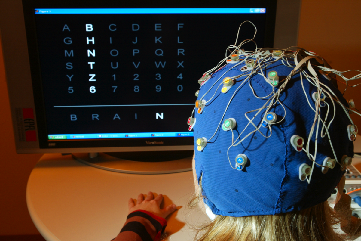
\includegraphics[width=1.7cm]{images/bci3.png}
\end{textblock*}%

\begin{textblock*}{2cm}(11.5cm,5.5cm)%
  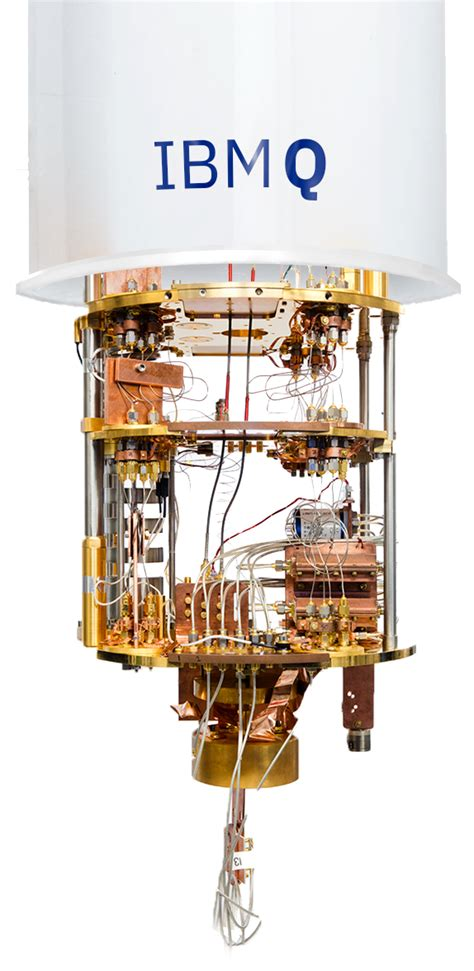
\includegraphics[width=.8cm]{images/ibmq.jpeg}
\end{textblock*}%

\begin{textblock*}{2cm}(9.2cm,6.5cm)%
  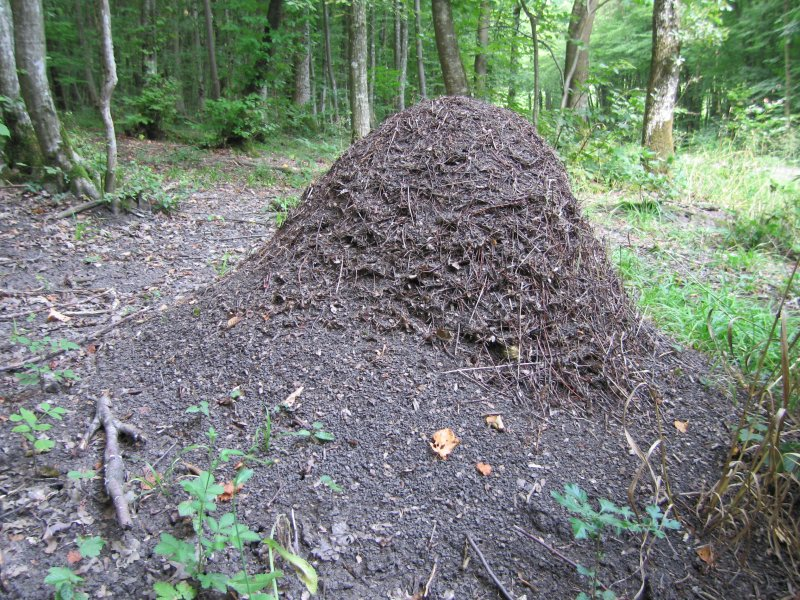
\includegraphics[width=2cm]{images/ants.jpeg}
\end{textblock*}%

\end{frame}

%%%%%%%%%%%%%%%%%%%%%%%%%%%%%%%%%%%%%%%%%%%%%%%%%%%%%%%%%%%%%%%%%%%%%%
\begin{frame}{Who are you?}

\end{frame}

%%%%%%%%%%%%%%%%%%%%%%%%%%%%%%%%%%%%%%%%%%%%%%%%%%%%%%%%%%%%%%%%%%%%%%
\begin{frame}{Lessons \& Labs}

  \begin{itemize}
%
    \item One plenary lesson
    \vspace{.5em}
    \begin{itemize}
      \item Labs organization
      \item Evaluations
      \item Outline
      \item Java basics
    \end{itemize}
%
    \vspace{2em}
    \item $\approx$10 labs
    \vspace{.5em}
    \begin{itemize}
      \item Introduce a (few) new concept(s) $\Rightarrow$ practice it
    \end{itemize}
%
    \vspace{2em}
    \item A final mini-project (Game)
%
  \end{itemize}

\end{frame}


%%%%%%%%%%%%%%%%%%%%%%%%%%%%%%%%%%%%%%%%%%%%%%%%%%%%%%%%%%%%%%%%%%%%%%
\begin{frame}{Evaluations}

  \begin{itemize}
    \item At the \textbf{beginning} of each Lab
    \begin{itemize}
      \item \textcolor{red}{You pass a MCQ @MOOTSE}
    \end{itemize}
%
    \vspace{2em}
    \item At the \textbf{end} of each Lab
    \begin{itemize}
      \item \textcolor{red}{You submit your work @GitLab/GitHub}
    \end{itemize}
%
    \vspace{2em}
    \item Final grade
    \begin{itemize}
      \item MCQs = 40\%
      \item Labs = 60\%
    \end{itemize}
%
  \end{itemize}

\end{frame}


%%%%%%%%%%%%%%%%%%%%%%%%%%%%%%%%%%%%%%%%%%%%%%%%%%%%%%%%%%%%%%%%%%%%%%
\begin{frame}{Outline}

  \begin{enumerate}
    \item Getting Started
    \item Files + Exceptions
    \item POJOs + Strings + Wrappers
    \item Collections
    \item Java8 : Lambdas, Streams
    \item OOP: Instances, Encapsulation, Inheritance, Polymorphism
    \item (Data Structures) Graphs
    \item (Data Base) JDBC
    \item (GUI) Swing
    \item (Algorithms) ConvexHull
    \item Mini-project [Multi-Threading, Introspection]
  \end{enumerate}

\end{frame}


\end{document}


%%% Local Variables:
%%% mode: latex
%%% TeX-master: t
%%% End: